%%%% 1. DOCUMENTCLASS %%%%
\documentclass[journal=tosc,final]{iacrtrans}
%%%% NOTES:
% - Change "journal=tosc" to "journal=tches" if needed
% - Change "submission" to "final" for final version
% - Add "spthm" for LNCS-like theorems


%%%% 2. PACKAGES %%%tsdss
\usepackage[left, pagewise,edtable]{lineno}
\usepackage{blt}
\usepackage{graphicx}
\usepackage{framed} 
\usepackage{xcolor}
\usepackage{tcolorbox}
\usepackage{xcolor} 
\colorlet{shadecolor}{gray!25}
\definecolor{mshadecolor}{rgb}{0.7421875,0.7421875,0.7421875}
\setlength{\OuterFrameSep}{10pt}
%%%% 3. AUTHOR, INSTITUTE %%%
\author{Moritz Rupp}
\institute{
  Hochschule Albstadt-Sigmaringen, Albstadt, Germany, \email{ruppmori@hs-albsig.de}
  
}



%%%% 4. TITLE %%%%
\title{Soziotechnische Lösungsansätze gegen Phishing}

\author{Moritz Rupp}

\begin{document}

\maketitle
\author

\begin{center}
\date{Sommersemester 2023 } 
\end{center}



%\vspace{15mm}
%%% 5. KEYWORDS %%%%s
\keywords{Social-Engineering \and Phishing \and IT-Security \and Container \and DNS }


%%%% 6. ABSTRACT %%%%s
\begin{abstract} Phishing zählt nach wie vor zu den häufigsten Methoden bei Cyberangriffen. Dabei werden versucht vertrauliche Informationen wie Passwörter oder Kreditkartennummern abzugreifen. Hierbei werden soziale Manipulationstechniken oder gefälschte Kommunikationskanäle genutzt, um das Vertrauen des Opfers zu gewinnen. Diese Arbeit untersucht Technische Lösungsansätze um dies vorzubeugen.  \end{abstract}

\newpage
\tableofcontents
\newpage

%%%% 7. PAPER CONTENT %%%%
\section{Einführung}
Phishing ist eine Form des betrügerischen Verhaltens im Internet, bei der Angreifer versuchen, sensible Informationen wie Benutzernamen, Passwörter, Kreditkartennummern oder andere persönliche Daten von Internetnutzern zu stehlen. Dies wird bewerkstelligt, indem Angreifer gefälschte Webseiten, E-Mails oder andere Kommunikationskanäle nutzen, um sich als vertrauenswürdige Quellen oder Organisationen auszugeben. Das Hauptziel des Phishings besteht immer darin, Opfer zu verleiten, ihre vertraulichen Informationen preiszugeben, indem sie beispielsweise auf einen gefälschten Link klicken, ihre Anmeldedaten auf einer gefälschten Website eingeben oder auf betrügerische E-Mails antworten.

Dazu nutzen Phishing-Angriffe oft soziale Manipulationstechniken, um das Vertrauen der Opfer zu gewinnen. Dies kann beispielsweise durch die Nachahmung von bekannten Unternehmen, Regierungsbehörden oder Finanzinstituten erfolgen. Die Angreifer verwenden entsprechende Sprache, gefälschte Logos und weitere Taktiken, um ihre gefälschten Kommunikationen authentisch wirken zu lassen.

Ein erfolgreicher Phishingangriff hat schwerwiegende Konsequenzen für die Opfer. Durch den Diebstahl persönlicher Daten können die Angreifer Identitätsdiebstahl begehen, finanziellen Schaden anrichten oder die gestohlenen Informationen für weitere kriminelle Aktivitäten nutzen. Darüber hinaus kann Phishing das Vertrauen der Benutzer in Online-Dienste und elektronische Kommunikation insgesamt untergraben.

Die Bekämpfung von Phishing erfordert eine Kombination aus technischen Lösungen, Benutzererziehung und rechtlichen Maßnahmen. Dies umfasst beispielsweise die Implementierung von Sicherheitsprotokollen wie E-Mail-Authentifizierung, Anti-Phishing-Filtern und Phishing-Warnungen in Webbrowsern. Die Sensibilisierung der Benutzer für Phishing-Techniken und die Förderung bewusster Online-Sicherheitspraktiken spielen ebenfalls eine wichtige Rolle bei der Verringerung des Risikos von Phishing-Angriffen.\\ Die Kombination von technischen und sozialen Komponenten und deren Abhängikeiten, kann als Sozio-technisches System bezeichnet werden. Die Strukturierung bzw. Beschreibung von solch einem System im Context von Phishing, kann hilfreich sein um die komplexe Landschaft aus Angriffvektoren und Präventivmaßnahmen richtig einordnen zu können. Diese Arbeit behandelt Sozio-technische Systeme  als Lösungsansatz gegen Phishing Angriffe. Dafür wird im ersten Schritt ein Sozio-technisches System definiert und auf Phishing angewand. Anschließend werden die teilkomponenten wie soziale und technische Lösungen vorgestellt und abschließend als gesamte Lösung zusammengeführt. 


\newpage

\section{Soziotechnische Systeme}
Ein soziotechnisches System ist ein Konzept, das die Wechselwirkung zwischen sozialen und technologischen Elementen in einer bestimmten Umgebung oder Organisation beschreibt. Konkret wird die Tatsache betrachtet, dass in vielen Bereichen und Systemen ein Zusammenspiel sowie eine Abhängigkeit zwischen Menschen und Technologien besteht. Zudem wird festgestellt das die Implementierung von Technologien nicht isoliert von sozialen, kulturellen oder organisatorschen Aspekten betrachtet werden kann. Stattdessen besteht selbst in vermeintlich rein technologischen Prozessen immer eine Abhängigkeit von Menschlichen, irrationalen Einflüssen.\\
Es ist möglich nahezu alle adaptiven Systeme als Soziotechnische Systeme zu modellieren. Darunter fallen beispielsweise Flugkontrollsysteme, Social-Media Plattformen, Krankenhausinformationssysteme oder Bildungseinrichtungen.\\
In Figure 1 wird ein Arbeitssystem als Soziotechnisches System dargestellt.
\begin{figure}[h]
\caption{Soziotechnisches System}
\begin{center}
 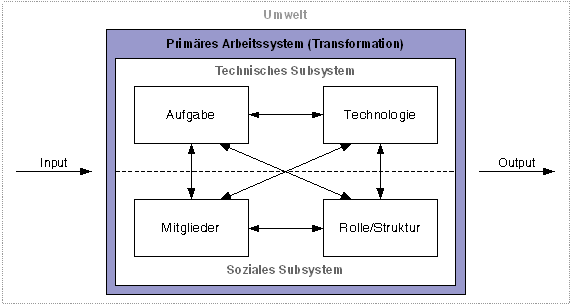
\includegraphics[scale=0.5]{sozio.png}
\end{center}
\end{figure}

Generell besteht ein Soziotechnisches System aus 2 Grundkomponenten.. Einer technische Teilkomponente und einer soziale Teilkomponente. Diese haben jeweils weitere Subkomponenten. Das Arbeitssystem besteht aus 2 sozialen Teilkomponenten. Mitgliedern sowie Rollen bzw. Strukturen. Zudem gibt es 2 Technische Teilkomponenten. Eine Technologie, und eine definierte Aufgabe. Alle Teile des Arbeitssystems haben Abhängigkeiten untereinander. Um nun aus einem Input einen Output zu erzeugen, müssen alle Teilkomponenten wechselseitig Interagieren. Fällt eines der Teilkomponenten aus, so ist das gesamte Arbeitssystem nicht mehr lauffähig. Die Technologie bearbeitet und verbessert die Arbeitsprozesse, während die Mitarbeiter ihr Fachwissen und ihre Erfahrung einbringen, um die Systeme zu steuern, zu überwachen und anzupassen. Die Effizienz und Qualität der Produktion hängen sowohl von der technischen Leistungsfähigkeit als auch von der Zusammenarbeit und Interaktion zwischen den Menschen und der Technologie ab. Die Betrachtung von Soziotechnischen Systemen ist wichtig, um die Auswirkungen technologischer Veränderungen auf die Arbeitswelt, die Gesellschaft und die Menschen zu verstehen. Es fördert einen ganzheitlichen Ansatz bei der Gestaltung und Implementierung von Technologie, bei dem soziale, organisatorische und technologische Faktoren berücksichtigt werden, um positive Ergebnisse und ein besseres Zusammenwirken von Mensch und Technologie zu erzielen. Insbesondere kann es helfen Problematiken in komplexen Systemen und Prozessen zu verstehen und richtig einzuordnen. Davon ausgehend können nun Lösungen entwickelt werden, die sowohl technische als auch soziale Aspekte miteinbeziehen.  
\newpage
\subsection{Phishing als Soziotechnisches System}
Ein Phishingangriff kann als ein Soziotechechnisches System modelliert werden. Die technischen Komponenten umfassen den Einsatz von Webseiten, E-Mails oder Kurznachrichtendiensten. Zu sozialen Komponenten zählen Angreifer sowie die Phishing Opfer. Des weiteren gibt es zwischen technischen und sozialen Komponenten Interaktionen und Abhängigkeiten. Um ein vollständiges System zu modellieren, muss zudem ein Ziel definiert werden. In Figure 2 ist Phishing als Soziotechnisches System modelliert.
\begin{center}
 \begin{figure}[h]
  \caption{Phishing als Soziotechnisches System}
  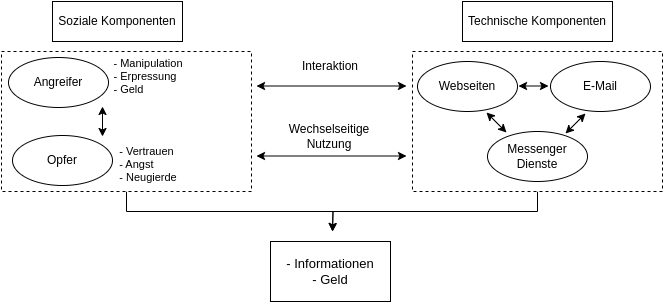
\includegraphics[scale=0.5]{syst.png}
 \end{figure}
\end{center}
Hierbei spielen die technischen Subkomponenten wie Webseiten, E-Mails und Messenger Dienste, wechselseitig mit den sozialen Subkomponenten wie Anreifer und Opfer zusammen, um an das Ziel, in Form von Informationen und Geld zu gelangen. Genauer  betrachtet bedient und missbraucht ein Phishingangriff die verschiedenen Komponenten. 

\begin{enumerate}
\item Technische Komponenten
\begin{itemize}
\item Mail-Server: Der Server, über den Phishing-E-Mails an potenzielle Opfer gesendet werden.
\item Phishing-Website: Eine gefälschte Website, die erstellt wurde, um die Opfer zur Preisgabe ihrer vertraulichen Informationen zu verleiten.
\item DNS-Server: Der Server, der die Domainnamen auflöst und es den Angreifern ermöglicht, gefälschte Domains zu verwenden.
\end{itemize}
\item Soziale Komponenten
\begin{itemize}
\item Phisher: Die Angreifer, welche die Phishing-Angriffe initiieren.
\item Opfer: Die Personen, die das Ziel der Phishing-Angriffe sind.
\end{itemize}
\end{enumerate}
Die Interaktion zwischen diesen Teilkomponenten sind beispielsweise der E-Mail Versand, die Nutzung von Webseiten oder die Preisgabe von Informationen. Diese Modellierung zeigt, die starke Interaktion zwischen den Komponenten. Zudem können Schwachstellen in diesem System identifiziert werden und geeignete Schutzmaßnahmen implementiert werden.
\subsection{Phishing-Prävention}
Durch die Betrachtung von Phishing als Soziotechechnische System, ist festzustellen das dieses eine hohe Anzahl an Abhängikeiten aufweist. Fällt eines der Subkomponenten aus, stoppt der Arbeitsprozess in Form des Phishing Angriffes. Wäre es möglich eines oder mehrere der Subkomponenten vollständig zu abzuschalten, könnte der Wirkungsgrad eines Phishingangriffes stark eingegrenzt werden. Dies gilt insbesondere für die Nutzung der Technischen Komponenten von seiten des Opfers. Diese werden als Einstiegskanal für die Interaktion zwischen Angreifer und Opfer genutzt. Könnte man also konkret die technische Teilkomponente wie ein E-Mail Client isolieren, wäre eine Interaktion deutlich schwerer. Auch Soziale Komponenten können verwendet  werden um einen Phishingangriff zu unterbinden. Die Effectivste Methode besteht jedoch darin, soziale und technische Teilkomponenten in einer soziotechnischen Lösung zusammenzuführen.
\section{Soziale Lösungsansätze}
Soziale Lösungsansätze gegen Phishing konzentrieren sich auf die Stärkung der Benutzer, die Sensibilisierung der Öffentlichkeit und die Förderung der Zusammenarbeit auf kollektiver Ebene. Diese Ansätze zielen darauf ab, das Wissen und die Fähigkeiten der Nutzer zu verbessern.
\section{Technische Lösungsansätze}
\subsection{DNS-Header}
\subsection{Container}
\section{Soziotechechnische Lösungen}
\bibliographystyle{alpha}
\bibliography{ref.bib}
\end{document}
